\usepackage[T2A]{fontenc}
\usepackage[utf8]{inputenc}
\usepackage[russian]{babel}

\usepackage{dsfont}

\newcommand{\bbS}{\mathds{S}}

\makeatletter
\newcommand{\xEC@family}[5]{%
  \DeclareFontShape{#1}{#2}{#3}{#4}%
  {<-5.5>#50500
   <5.5-6.5>#50600
   <6.5-7.5>#50700
   <7.5-8.5>#50800
   <8.5-9.5>#50900
   <9.5-10.5>#51000
   <10.5-11.5>#51095
   <11.5-13>#51200
   <13-16>#51440
   <16-18>#51728
   <18-21>#52074
   <21-26.88>#52488
   <26-32>#52986
   <32->#53583}{}}
\DeclareFontFamily{T2A}{cmr}{}
\xEC@family{T2A}{cmr}{m}{n}{larm}
\xEC@family{T2A}{cmr}{m}{sl}{lasl}
\xEC@family{T2A}{cmr}{m}{it}{lati}
\xEC@family{T2A}{cmr}{m}{sc}{lacc}
\xEC@family{T2A}{cmr}{bx}{n}{labx}
\xEC@family{T2A}{cmr}{b}{n}{larb}
\xEC@family{T2A}{cmr}{bx}{it}{labi}
\xEC@family{T2A}{cmr}{bx}{sl}{labl}
\xEC@family{T2A}{cmr}{bx}{sc}{laxc}
\xEC@family{T2A}{cmr}{m}{ui}{laui}
\makeatother

\title{\parbox{\linewidth}{\centering Исследование бифуркаций в трехатомных гидридах \\ методом классических траекторий}}

%\titlegraphic{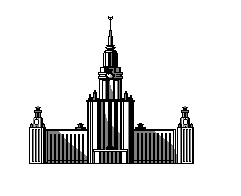
\includegraphics[width=7cm]{pictures/logo.jpg}}

\author{Финенко Артем}
\institute{МГУ им. М.В. Ломоносова}
